\documentclass{beamer}

\usepackage{hyperref}
\hypersetup{
  colorlinks = true
}
\usepackage[utf8]{inputenc}
\usepackage{amsmath}
\usepackage{amssymb}

% beamer
\setbeamertemplate{navigation symbols}{}

% Information to be included in the title page:
\title{ECE 590D-001, Reinforcement Learning at Scale}
\author{Jay Hineman, Ph.D.}
\institute{Geometric Data Analytics}
\date{2020}
 
 
 
\begin{document}
 
\frame{\titlepage}

\begin{frame}
  \frametitle{Sequential decision (intuition)}
  \begin{columns}[T]
    \begin{column}{.5\textwidth}
      \begin{itemize}
      \item MDP: {\em Markov decision process}
      \item {\em MDPs are a classical formalization of sequential decision
          making, where actions influence not just immediate rewards, but also subsequent
          situations, or states, and through those future rewards.}
      \end{itemize}
    \end{column}
    \begin{column}{.5\textwidth}
      \begin{figure}
        \label{fig:mdp-agent-env-loop}
        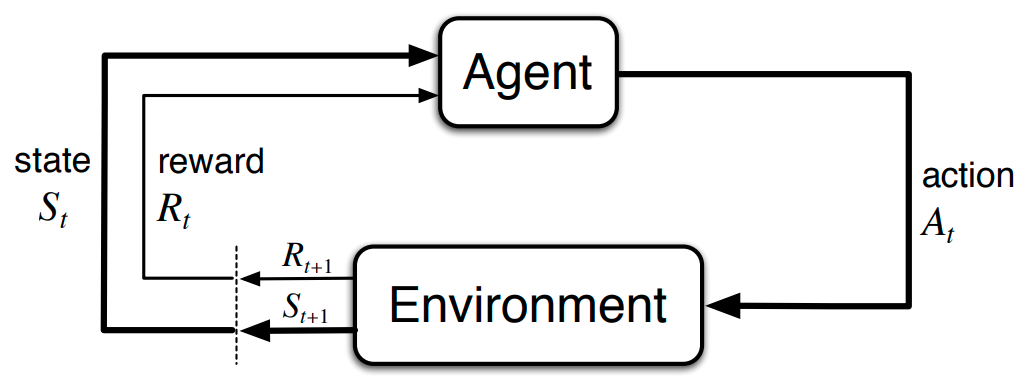
\includegraphics[width=\textwidth]{../images/agent-environment-loop.png}
        \caption{Agent-environment loop diagramming a Markov decision process.}
      \end{figure}
    \end{column}
 \end{columns}
\end{frame}

\begin{frame}
  \frametitle{Recycling robot {\em Example 3.3} \cite{Sutton2018}}
  \begin{columns}[T]
    \begin{column}{.5\textwidth}
      \begin{itemize}
      \item States: $\{\text{low},\text{high}\}$
      \item Actions: $\{\text{wait}, \text{search}, \text{recharge}\}$
      \item Transitions: <<board!!
      \end{itemize}
    \end{column}
    \begin{column}{.5\textwidth}
      \begin{figure}
        \label{fig:recycle-robot-mdp}
        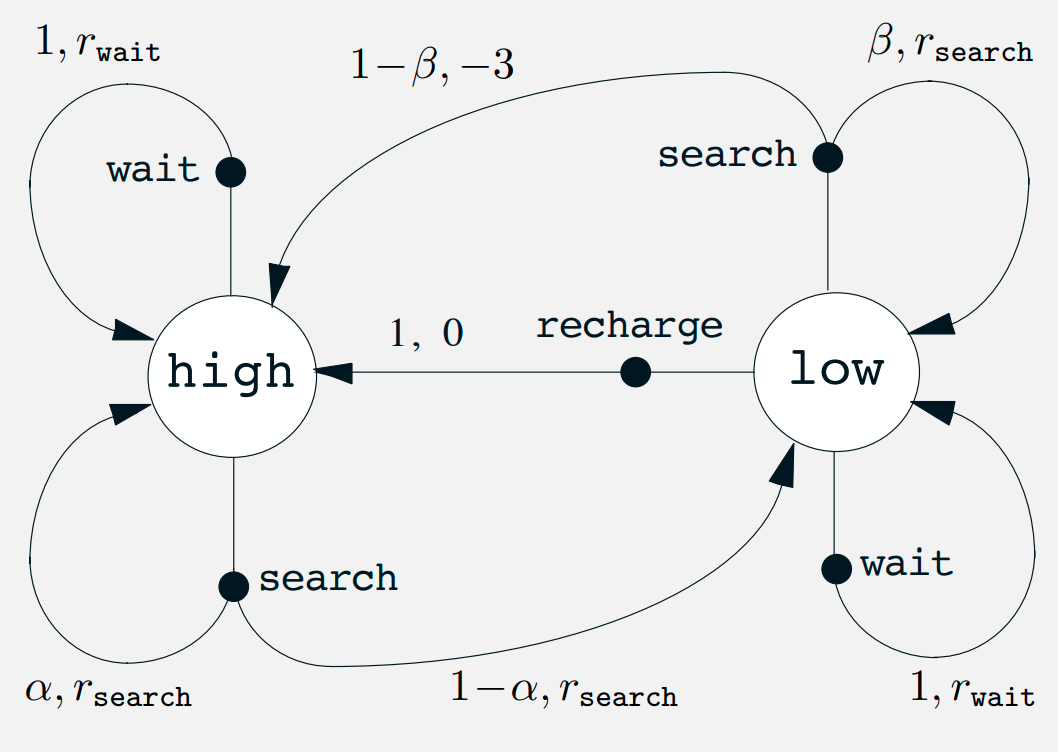
\includegraphics[width=\textwidth]{../images/sutton2018_recycle_robot.png}
        \caption{Diagram of MDP for \cite{Sutton2018} recycling robot example
          (page 52, Example 3.3).}
      \end{figure}
    \end{column}
  \end{columns}
\end{frame}

\begin{frame}
  \frametitle{Pole Balancing (cart-pole) {\em Example 3.4} \cite{Sutton2018}}
  \begin{columns}[T]
    \begin{column}{.5\textwidth}
      \begin{itemize}
      \item States: $\phi \in [0, \pi]$
      \item Actions: accelerate cart left or right
      \item Transitions: an ODE
      \end{itemize}
    \end{column}
    \begin{column}{.5\textwidth}
      \begin{figure}
        \label{fig:cart-pole}
        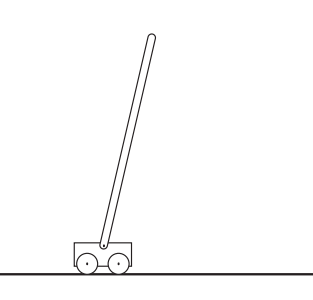
\includegraphics[width=.8\textwidth]{../images/sutton2018_cartpole.png}
        \caption{A {\em classic} problem in control: cart-pole/pole balancer/broom balancer.}
      \end{figure}
    \end{column}
  \end{columns}
\end{frame}
  
\begin{frame}
  \frametitle{Gridworld {\em Example 3.5} \cite{Sutton2018}}
  \begin{columns}[T]
    \begin{column}{.5\textwidth}
      \begin{itemize}
      \item States: $\{(x,y): x = 0,1, \ldots, m, \ y = 0,1,, \ldots n\}$
      \item Actions: $\{\text{N}, \text{E}, \text{S}, \text{W}\}$
      \item Transitions: <<board!!
      \end{itemize}
      \begin{figure}
        \label{fig:gridworld-3.5}
        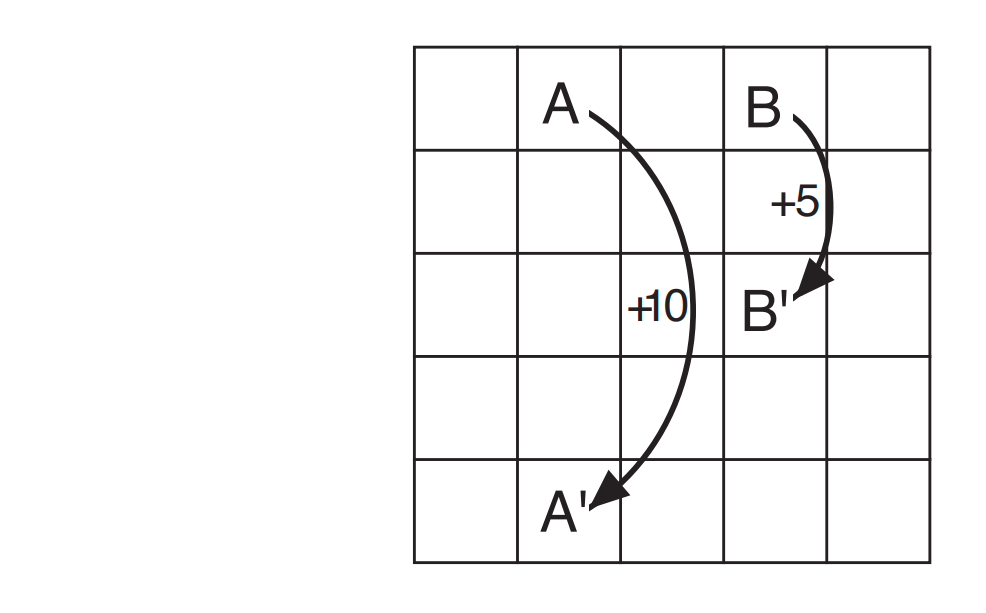
\includegraphics[width=\textwidth]{../images/sutton2018_gridworld3_5.png}
        \caption{5-by-5 gridworld with 2 distinguished states $A$ and $B$.}
      \end{figure}
    \end{column}
    \begin{column}{.5\textwidth}
      \begin{figure}
        \label{fig:gridworld-action-rand-pol}
        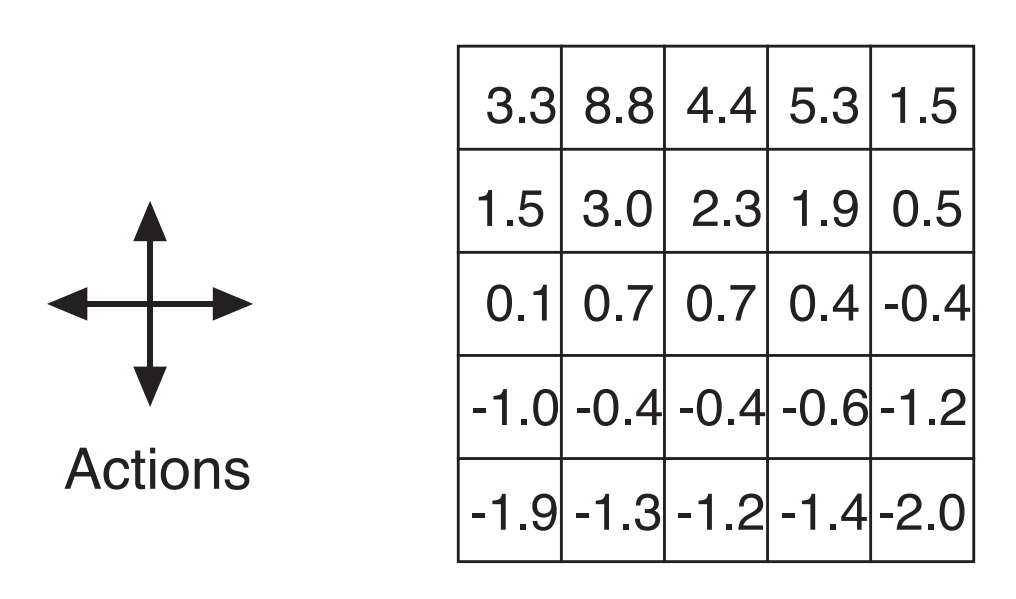
\includegraphics[width=\textwidth]{../images/sutton2018_gridworld_rand_pol_val.png}
        \caption{Actions representation and State-Value function for uniform random policy.}
      \end{figure}
    \end{column}
  \end{columns}
\end{frame}

\begin{frame}
  \frametitle{Mathematical details \cite{Sutton2018}}
  {\bf Following Sutton and Barto \cite{Sutton2018}}
  \begin{itemize}
  \item $t=\text{time/iteration}$, $s, S_t \in \mathcal{S} = \text{states}$, $a, A_t \in \mathcal{A}(s) = \text{actions at state}$, $r, R_{t+1} \in \mathbb{R} = \text{rewards}$,
    $S_0, A_0, R_1, S_1, A_1, R_2, S_2, A_2, R_3, \ldots = \text{trajectory}$
  \item $\text{transition function} = p(s', r'| s, a) := \text{Prob}\{S_t = s', R_t = r | S_{t-1} = s, A_{t-1} = a\}$
  \item {\bf probability fact:} $\sum_{s',r} p(s',r | s, a) = 1$ for all $s \in \mathcal{S}, a \in \mathcal{A}(s)$
  \item {\bf return and discounted return:} $G_t = R_{t+1} + R_{t+2} + R_{t+3} + \cdots + R_{T}$ and $G_t = R_{t+1} + \gamma R_{t+2} + \gamma^2 R_{t+3} + \cdots$
  \item {\bf ((board work))} from \cite{Sutton2018}
  \end{itemize}
\end{frame}

\begin{frame}
  \frametitle{Policy, value, and action value functions}
  \begin{itemize}
  \item {\bf value and action-value functions:} functions of states (or of state–action pairs) that estimate how good it is for the agent to be in a
    given state (or how good it is to perform a given action in a given state).
  \item {\bf policy:} a policy is a mapping from states to probabilities of selecting each possible action.
  \item {\bf ((board work))} from \cite{Sutton2018}
  \end{itemize}
\end{frame}

\begin{frame}
  \frametitle{Mathematical specification of value and action-value}
  \begin{equation}
    \begin{aligned}
      q_\pi(s) &= \mathbb{E}_\pi[G_t|S_t = s, A_t = a] \\
      &= \mathbb{E}_\pi [\sum_{k=0} \gamma^k R_{(t + 1) + k} | S_t = s, A_t = a ], s \in \mathcal{S} \\
      &= \text{Value of $s$ given the policy $\pi$} \\
      v_\pi(s) &= \mathbb{E}_\pi[G_t|S_t = s] \\
      &= \mathbb{E}_\pi [\sum_{k=0} \gamma^k R_{(t + 1) + k} | S_t = s ] \\
      &= \text{action-value or $q$-value of $s,a$ given the policy $\pi$}
    \end{aligned}
  \end{equation}
  \begin{itemize}
  \item {\bf ((board work))} on {\em Bellman equation} for $v_\pi$ from \cite{Sutton2018}
  \end{itemize}
\end{frame}

\begin{frame}
  \frametitle{Spinning up's \href{https://spinningup.openai.com/en/latest/spinningup/rl_intro2.html}{Taxonomy}}
  \begin{figure}
    \label{fig:deep-rl-taxonomy}
    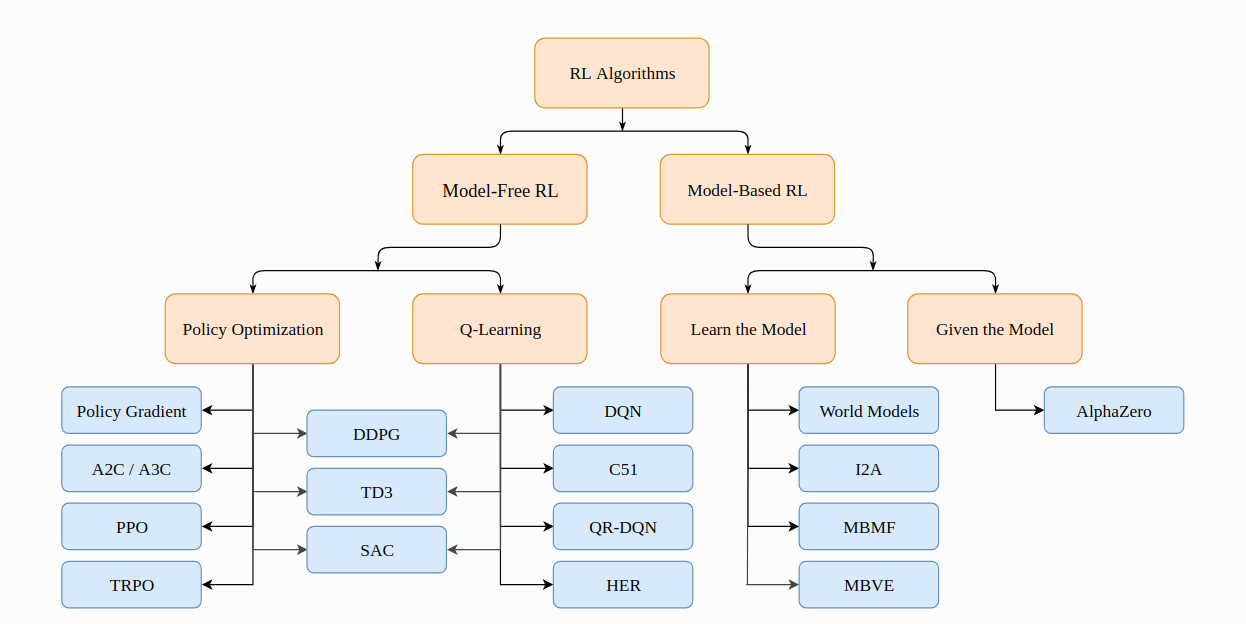
\includegraphics[width=\textwidth]{../images/spinup_rl_taxonomy.png}
    \caption{Non-exhaustive, but nice starting Taxonomy of (deep) RL methods. See also:
      \href{https://spinningup.openai.com/en/latest/spinningup/rl_intro2.html\#citations-below}{citations.}}
  \end{figure}
\end{frame}

\end{document}

% two column sample 
\begin{frame}
\frametitle{A frame}
  \begin{columns}[T]
    \begin{column}{.5\textwidth}
     \begin{block}{Your textblock}
% Your text here
    \end{block}
    \end{column}
    \begin{column}{.5\textwidth}
    \begin{block}{Your image}
% Your image included here
    \includegraphics[<options, e.g. width=\textwidth>]{<your image file>}
    \end{block}
    \end{column}
  \end{columns}
\end{frame}